\documentclass[runningheads]{llncs}
\usepackage{fontspec,xeCJK}
\setCJKmainfont{Noto Serif CJK SC}
\setCJKsansfont{Noto Sans CJK SC}
\usepackage{amsmath,amssymb,booktabs,graphicx,multirow}
\usepackage[hidelinks]{hyperref}
\renewcommand{\abstractname}{摘要}
\renewcommand{\keywordname}{关键词：}
\renewcommand{\figurename}{图}
\renewcommand{\tablename}{表}
\renewcommand{\refname}{参考文献}
\spnewtheorem{zhproposition}{命题}{\bfseries}{\itshape}
\spnewtheorem*{zhproof}{证明}{\itshape}{\rmfamily}
\begin{document}
\title{事后之见并非机会：\\延迟反馈下风险约束标签获取的结果前价值}
\titlerunning{事后之见并非机会}
\author{匿名作者}
\authorrunning{匿名作者}
\institute{匿名机构}
\maketitle
\begin{abstract}
在信贷及其他决策系统中，标签需要通过采取有风险的行动来获取，结果延迟到达，而风险预算限制了哪些标签集合是可行的。本文研究：何时决定学习价值的是可行集合的\emph{组成}而非其\emph{规模}，以及策略在结果揭晓之前能够实现其中多少价值。我们给出同一状态下的数量—组成分解；给出一个闭式阈值，在固定预算下，待反馈信息超过该阈值时偏好集合发生反转；并将结果揭晓后的提升空间分解为不可部署的\emph{先见}项和\emph{结果前}项，后者在结果概率已知时可直接估计。一个基于机制设计的参考策略 DC-PRISM 作为研究工具。在受控世界中，结果揭晓后提升空间的 83\% 可在结果到达前实现；相对风险基准，DC-PRISM 将期望 Brier 损失降低 $12.2\times10^{-3}$，而获取的标签数约为一半。在真实信贷协变量上，同一提升空间的 61--90\% 属于先见；覆盖缺口会扩大结果前部分，点估计价值代理能较好地对其排序，但驱动受控收益的保守层在 84--95\% 的状态中返回基准集合。在四个信贷队列上进行的在线回放（包括工程化与自然两种候选流、八个对照策略）未发现决定性差异。这些结果将事后之见与可部署的机会区分开来，并揭示了在利用有利信息几何时存在的保守性权衡。
\keywords{选择性标签 \and 风险约束获取 \and 延迟反馈 \and 主动学习 \and 信用风险}
\end{abstract}

\section{引言}
\label{sec:intro}
贷款机构只能观察到其批准的申请的还款结果，因此未来学习可用的数据取决于早先的决策~\cite{lakkaraju2017selective,wei2021selective}。每一次批准同时也是一次损失敞口。当结果延迟到达时，学习器还必须考虑那些已经做出但尚未结清的决策。因此，此类系统中的标签获取同时涉及风险预算、对总体的不完全覆盖，以及已经承诺但仍在等待的信息。

风险预算决定哪些标签集合是可行的，但并不决定哪个可行集合最有价值。主动学习与实验设计依据观测对预测的预期贡献来选择样本~\cite{cohn1996active,yu2006transductive,settles2009active}，近期的准则则以 Fisher 信息、预测信息或下游损失为目标~\cite{ash2021fishing,bickfordsmith2023prediction,huang2026loss}。在风险预算下，一个信息丰富但敞口较大的观测可能挤占若干个廉价观测，因此组成与数量之间存在直接权衡。待反馈的结果会再次改变这一比较，因为某些方向上的信息已经在途中。

本文是对这一权衡的机制研究。我们提出三个问题：（i）相对于以数量为导向的基准，数量与组成分别如何贡献于可行集合的实际收益？（ii）在预算不变的情况下，待反馈信息何时会反转偏好的组成？（iii）结果到达\emph{之后}可见的机会中，有多少是任何策略在结果到达\emph{之前}就能实现的？第三个问题之所以重要，是因为获取策略的实证研究经常把所选集合与事后最优集合进行比较。这种事后提升空间混合了两类价值：利用手头信息即可实现的价值，以及需要知道隐藏训练标签才能实现的价值。

\paragraph{贡献。}
\begin{itemize}
\item \textbf{机制分析。}给出同一状态下的数量—组成分解，以及一个闭式阈值：在相同预算下，当方向性待反馈信息超过该阈值时，较小的可行集合更可取（第~\ref{sec:mechanism}~节）。
\item \textbf{事后价值与结果前价值。}将结果揭晓后的提升空间分解为先见项与结果前选择项，并给出一个区间夹逼的蒙特卡洛估计量，使得在结果概率已知时这些项可以被测量（第~\ref{sec:opportunity}~节）。
\item \textbf{分层证据。}在受控世界、带配对覆盖干预的真实信贷协变量、以及四个信贷队列上的延迟回放（工程化与自然候选流，八个对照策略）上进行预注册实验。实验表明，受控世界中的机会大部分可部署，而真实协变量上的机会主要是先见；并将剩余差距定位为决策规则中的保守性权衡（第~\ref{sec:controlled}--\ref{sec:replay}~节）。
\end{itemize}
我们作为研究工具使用的策略 DC-PRISM 由该机制推导而来：它使用考虑待反馈信息、按目标加权的信息量，将可行集合与数量基准进行比较（第~\ref{sec:policy}~节）。我们并不声称它在真实数据上优于简单的基于信息的基线；实验展示了它在何处有效、在何处无效，以及原因。

\section{问题设定}
\label{sec:setting}
在第 $t$ 轮，学习器观测到已标注历史 $D_t$、待反馈获取样本的协变量 $O_t$、未标注候选池 $C_t$ 以及目标协变量 $Q_t$。候选 $i$ 具有可见敞口 $e_i\geq0$ 和一个二元不利结果 $Y_i$，后者仅在获取并经过反馈延迟后才揭晓。合法策略利用可见信息 $\mathcal H_t$ 选择 $S_t\subseteq C_t$；$O_t$ 与 $C_t$ 中的结果保持隐藏。学习效果以 Brier 分数~\cite{brier1950verification}衡量。对固定状态，$L(S;Y)$ 表示在 $D\cup O\cup S$ 上拟合后的测试损失，其中 $Y$ 汇集了 $O$ 与 $S$ 的隐藏训练结果。

\paragraph{风险可行集合。}设 $q_i\in[0,1]$ 为选择时可用的风险分数，$\ell=\log(1/\alpha)$；当 $q\le1/2$ 时 $\phi(q)=q(1-q)$，否则 $\phi(q)=1/4$。对非空 $S$，
\begin{equation}
 R_\alpha(S)=\sum_{i\in S}e_iq_i+\Big(2\ell\sum_{i\in S}e_i^2\phi(q_i)\Big)^{1/2}+\frac{\ell}{3}\max_{i\in S}e_i,
 \label{eq:envelope}
\end{equation}
$R_\alpha(\varnothing)=0$，且 $\mathcal A_t=\{S\subseteq C_t:R_\alpha(S)\le B_t\}$。若在给定 $\mathcal H_t$ 的条件下，被选样本的结果是独立的 Bernoulli 变量且 $p_i\le q_i$，则由次伽马（sub-gamma）界~\cite{boucheron2013concentration}可得 $\Pr\{\sum_{i\in S}e_iY_i>R_\alpha(S)\mid\mathcal H_t\}\le\alpha$。我们的实验使用经验 Wilson/Laplace 分数，此时上述条件无法保证；我们将~\eqref{eq:envelope} 作为所有策略共享的操作性可行域。

\paragraph{数量基准。}基准 $M_K\in\mathcal A_t$ 最大化集合基数，并以较小包络值打破平局；$K=|M_K|$。小规模候选池采用穷举；较大候选池采用按敞口分层的搜索并配合基数上界。

\section{机制分析}
\label{sec:mechanism}
\subsection{数量与组成}
对于所选的 $S$，$|S|=k\le K$，令 $M_k$ 为大小为 $k$ 的可行风险排序基准（当 $k=K$ 时复用 $M_K$）。在相同的 $D\cup O$ 与实现结果下，
\begin{equation}
\begin{gathered}
 Q_k=L(M_k;Y)-L(M_K;Y),\qquad C_k=L(M_k;Y)-L(S;Y),\\
 J=L(M_K;Y)-L(S;Y)=C_k-Q_k.
\end{gathered}
 \label{eq:decomposition}
\end{equation}
$Q_k$ 比较两个规模不同的风险基准；$C_k$ 比较规模相同的集合。$J>0$ 表示组成的贡献超过了数量项的补偿。$Q_k$ 不一定为正：更大的基准可能具有更高的测试损失。

\subsection{方向性待反馈信息}
考虑一个二参数线性高斯模型，精度矩阵 $H=\operatorname{diag}(h_1,h_2)$，目标权重 $G=\operatorname{diag}(g_1,g_2)$，损失为 $\operatorname{tr}(GH^{-1})$。待反馈观测沿方向~1 增加精度 $o\ge0$。数量基准沿方向~1 增加精度 $a$；一个较小的替代集合沿方向~2 增加精度 $b$。当 $o$ 变化时，两者都保持可行。

\begin{zhproposition}[方向性偏好反转]
替代集合相对基准的收益为
$J(o)=\frac{g_2b}{h_2(h_2+b)}-\frac{g_1a}{(h_1+o)(h_1+o+a)}$，它关于 $o$ 严格递增。记 $v_2=g_2b/[h_2(h_2+b)]$，则替代集合更优当且仅当
\begin{equation}
 o>o^*=\tfrac12\big(-a+\sqrt{a^2+4g_1a/v_2}\big)-h_1 .\label{eq:threshold}
\end{equation}
\end{zhproposition}
\begin{zhproof}
两者的损失分别为 $g_1/(h_1+o+a)+g_2/h_2$ 与 $g_1/(h_1+o)+g_2/(h_2+b)$；相减得到 $J(o)$，其导数 $g_1a[2(h_1+o)+a]/[(h_1+o)^2(h_1+o+a)^2]$ 为正。求解 $(h_1+o)(h_1+o+a)>g_1a/v_2$ 即得~\eqref{eq:threshold}。\qed
\end{zhproof}
该反转发生在固定的敞口预算之下。取 $h_j=g_j=1$，方向~1 上四个单位信息标签（$a=4$）对比方向~2 上一个标签（$b=1$），$\alpha=0.1$，$q=0.1$；基准标签每个敞口为 $0.1$，替代标签敞口为 $0.1624$，此时两种行动的包络值均为 $B\approx0.2455$，且任何混合都不可行。在 $o=0$ 时基准更优（损失 $1.20$ 对 $1.50$），在 $o=1$ 时替代集合更优（$1.17$ 对 $1.00$），阈值 $o^*\approx0.464$（图~\ref{fig:reversal}）。待反馈信息降低了在基准轴上再增加一个观测的价值，而另一轴不受影响；因此，候选样本的价值必须相对于历史\emph{加上}待反馈信息来评估。

\begin{figure}[t]
 \centering
 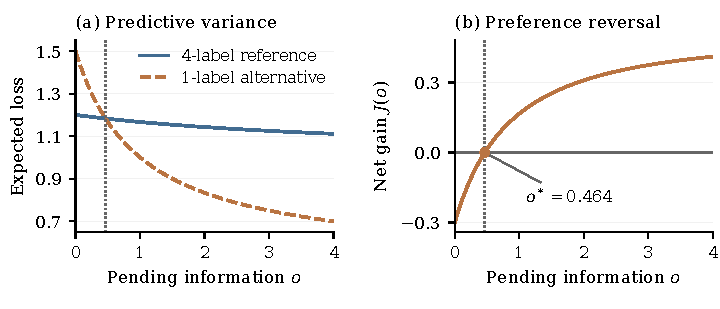
\includegraphics[width=0.92\linewidth]{figures/fig_information_reversal.pdf}
 \caption{固定风险预算下二方向模型中的偏好反转。单标签替代集合在 $o^*\approx0.464$ 处开始更优。}
 \label{fig:reversal}
\end{figure}

\subsection{事后机会与结果前机会}
\label{sec:opportunity}
固定 $\mathcal H$，以及一个由可见信息构造、包含 $M=M_K$ 的有限集合族 $\mathcal F$。令 $L(S,Y)$ 对测试标签噪声积分，但保留隐藏训练标签 $Y$。定义
\begin{align}
 H_{\mathrm{post}}&=\mathbb E\big[L(M,Y)-\min_{S\in\mathcal F}L(S,Y)\mid\mathcal H\big],\\
 H_{\mathrm{pre}}&=\mathbb E[L(M,Y)\mid\mathcal H]-\min_{S\in\mathcal F}\mathbb E[L(S,Y)\mid\mathcal H].
\end{align}
由于最小值的期望不超过期望的最小值，有 $H_{\mathrm{post}}\ge H_{\mathrm{pre}}\ge0$。对于在 $\mathcal F$ 中进行选择的任意合法策略 $\pi$，记其期望收益为 $G_\pi=\mathbb E[L(M,Y)-L(\pi,Y)\mid\mathcal H]$，则
\begin{equation}
 H_{\mathrm{post}}-G_\pi=\underbrace{H_{\mathrm{post}}-H_{\mathrm{pre}}}_{\text{先见}}+\underbrace{H_{\mathrm{pre}}-G_\pi}_{\text{结果前选择差距}} .\label{eq:opportunity}
\end{equation}
先见项对任何可部署策略都不可得；只有第二项可以通过更好的选择来缩小。与实现后最优集合进行的事后比较估计的是 $H_{\mathrm{post}}$，因而高估了可部署的机会。

\paragraph{估计。}当结果概率 $p$ 已知时，我们抽取隐藏训练标签的 $R$ 个重复样本 $Y^{(r)}$，并使用公共随机数在所有重复样本上评估每个 $S\in\mathcal F$。$H_{\mathrm{post}}$ 可被无偏估计。插值估计（plug-in）$\widehat H_{\mathrm{pre}}$ 对重复样本均值取最小，由于在噪声上做选择而向上偏。两折交叉拟合估计在偶数重复样本上选择 $S^\star$、在奇数重复样本上评估（反之亦然），其偏差向下。二者共同夹逼 $H_{\mathrm{pre}}$，而 $H_{\mathrm{post}}-\widehat H_{\mathrm{pre}}^{\text{plug-in}}$ 是先见项的保守估计。

\section{DC-PRISM：一个基于机制的参考策略}
\label{sec:policy}
DC-PRISM 以可行集合在历史与待反馈信息之上所能带来的目标加权 Brier 降低量来评估该集合，并将其与数量基准比较。采用 $\ell_2$ 正则化逻辑回归模型，记 $\bar x=(1,x^\top)^\top$，$p_\theta(x)=\sigma(\bar x^\top\theta)$，$w_\theta=p_\theta(1-p_\theta)$，令
\begin{gather*}
 H_{D+O}(\theta)=\Lambda+\!\!\sum_{i\in D\cup O}\!\!w_\theta(x_i)\bar x_i\bar x_i^\top,\qquad
 A_S(\theta)=\sum_{i\in S}w_\theta(x_i)\bar x_i\bar x_i^\top,\\
 G_Q(\theta)=\tfrac1{|Q|}\sum_{j\in Q}w_\theta(x_j)^2\bar x_j\bar x_j^\top,
\end{gather*}
\begin{equation}
 V_\theta(S)=\operatorname{tr}\!\big[G_Q(\theta)\{H_{D+O}(\theta)^{-1}-(H_{D+O}(\theta)+A_S(\theta))^{-1}\}\big].\label{eq:value}
\end{equation}
$V_\theta$ 是目标 Brier 降低量的局部二次代理，思路与直推式设计和预测信息获取~\cite{yu2006transductive,bickfordsmith2023prediction}一致；待反馈样本的协变量以不带标签的形式进入 $H_{D+O}$，这恰好对应命题中对已覆盖方向的折减。

\paragraph{决策规则。}候选集合族包含 $M_K$、按单位包络成本价值排序的前缀、按价值排序的前缀，以及保留 $M_K$ 部分元素的交换集合，所有集合均按~\eqref{eq:envelope} 检验可行性。对 $m=1,\dots,M$，抽取 $\theta^{(m)}\sim\mathcal N(\widehat\theta,H_D^{-1})$~\cite{mackay1992practical}，候选样本的曲率以 $\exp[-0.45\{\bar x_i^\top(\theta^{(m)}-\widehat\theta)\}^2]$ 进行阻尼，并令 $a_m=\max\{V_m(M_K),10^{-6}\}$，
\begin{equation}
 Z(S)=\operatorname{quantile}_{0.2}\Big\{\tanh\frac{V_m(S)-a_m}{2.5a_m}\Big\}_m-0.22\,\frac{(K-|S|)_+}{\max(K,1)} .\label{eq:score}
\end{equation}
若 $Z>0.08$，DC-PRISM 选择 $\arg\max Z$，否则选择 $M_K$。低分位数、曲率阻尼和基准归一化使该规则具有\emph{保守性}：较小的集合必须在大多数参数抽样下都优于 $M_K$。风险分数 $q$ 由两部分组合而成：对拟合历史风险的上半部分做单侧 Wilson 调整~\cite{wilson1927probable}，以及 40 次 Laplace logit 抽样上的高分位数。所有常数均在本文报告的实验之前固定；第~\ref{sec:controlled}~节报告其敏感性。

\paragraph{对照策略。}所有策略共享相同的状态、$q$、数值预算与~\eqref{eq:envelope}。\emph{Safe-MinRisk} 返回 $M_K$。\emph{固定数量（Fixed count）}按点估计价值选择 $\lceil0.75K\rceil$ 个标签。\emph{Fisher-cost} 按单个观测的参数方差降低量除以敞口成本进行贪心装填。另有四个基线持续贪心装填，直到不再有可行候选：\emph{Random}（随机）；\emph{Uncertainty}（不确定性），按 $\widehat p(1-\widehat p)$ 排序~\cite{lewis1994sequential}；\emph{BAIT-greedy}，以候选池 Fisher 矩阵 $F_Q$ 对 $\operatorname{tr}(F_Q(H_{D+O}+A_S)^{-1})$ 做前向贪心~\cite{ash2021fishing}；以及 \emph{TargetVar-greedy}，对~\eqref{eq:value} 做前向贪心，它是 EPIG 风格的 Laplace 近似~\cite{bickfordsmith2023prediction}，使用 DC-PRISM 的代理，但不含其基准比较、分位数、惩罚项或门限。

\section{受控实验证据}
\label{sec:controlled}
\paragraph{设计。}每个世界包含六个特征、80 个覆盖范围狭窄的历史标签、22 个集中在同一方向上的待反馈获取、24 个候选、180 个目标点和 240 个测试点。候选分组包括：低风险核心观测、与待反馈方向一致的观测、位于另外两个预测方向上的观测，以及辅助尾部观测——后者的结果服从逻辑回归模型无法表示的分段机制。所有选择均在读取任何隐藏标签之前锁定。下述每项研究在运行前都固定了世界数量、随机种子、比较族以及 $5\times10^{-4}$ Brier 的实质效应阈值。我们报告配对均值及 95\% Bonferroni 同时 $t$ 区间，并在每个比较族内进行 Holm 校正检验~\cite{holm1979simple}。

\paragraph{实际收益及其构成。}在 128 个存档世界中，DC-PRISM 以 $3.27$ 个标签取得 $0.1202$ 的 Brier 分数，而使用六个标签的 Safe-MinRisk 与使用四个标签的固定数量规则均为 $0.1367$（配对超额 $16.5\times10^{-3}$，95\% CI $[11.0,22.0]\times10^{-3}$）。同一状态分解给出 $C_k=16.3$，$Q_k=-0.19$，$J=16.4$（$\times10^{-3}$）：收益来自组成，并且较小的风险基准并不劣于较大的基准。

\paragraph{新世界，事前终点。}在 128 个新生成的世界中，我们以期望 Brier 评估每个策略：对测试标签噪声精确积分，对训练标签噪声在 128 个重复样本上积分（表~\ref{tab:controlled}）。DC-PRISM 损失最低。它相对 Safe-MinRisk（$12.2$，同时区间 $[7.6,16.8]$）、Fisher-cost（$17.8$，$[13.2,22.4]$）、Random（$9.7$，$[5.1,14.4]$）和固定数量（$9.6$，$[5.1,14.2]$）的收益是实质性的。它相对 Uncertainty、BAIT-greedy 和 TargetVar-greedy 的收益为 $2.7$--$4.2$，但这些区间包含零（均为 $\times10^{-3}$）。

\begin{table}[t]
\caption{新受控世界（128 个）：事前期望 Brier、平均标签数，以及 DC-PRISM 的收益和 95\% 同时区间（$\times10^{-3}$；正值有利于 DC-PRISM）。}
\label{tab:controlled}
\centering\small
\begin{tabular}{lrrr}
\toprule
策略 & 期望 Brier & 标签数 & DC-PRISM 的收益 \\
\midrule
Safe-MinRisk & 0.1384 & 6.00 & $12.2$ [$7.6$, $16.8$] \\
固定数量 & 0.1358 & 5.00 & $9.6$ [$5.1$, $14.2$] \\
Random & 0.1359 & 3.54 & $9.7$ [$5.1$, $14.4$] \\
Uncertainty & 0.1304 & 2.81 & $4.2$ [$-0.8$, $9.2$] \\
Fisher-cost & 0.1440 & 2.67 & $17.8$ [$13.2$, $22.4$] \\
BAIT-greedy & 0.1289 & 2.22 & $2.7$ [$-1.3$, $6.7$] \\
TargetVar-greedy & 0.1290 & 2.19 & $2.8$ [$-1.2$, $6.9$] \\
DC-PRISM & \textbf{0.1262} & 3.12 & -- \\
\bottomrule
\end{tabular}
\end{table}

\paragraph{机会。}此处 $H_{\mathrm{post}}=22.2\times10^{-3}$，$H_{\mathrm{pre}}\in[18.4,18.5]\times10^{-3}$：事后提升空间的 83\% 可在结果到达之前实现，DC-PRISM 获取了其中的三分之二（图~\ref{fig:opportunity} 左）。DC-PRISM 在 96\% 的世界中偏离 $M_K$。

\paragraph{组件与常数。}在一次每次只改变一个组件的公共比较族研究中，低分位数与待反馈重评分带来的收益均值为正，分别为 $3.9$ 和 $3.0\times10^{-3}$，但区间包含零；门限与数量惩罚的均值在 $\pm0.3\times10^{-3}$ 以内。改变任一单个常数（分位数 $0.1$--$0.5$、惩罚 $0$--$0.44$、门限 $0$--$0.16$、阻尼 $0$--$0.9$、tanh 尺度 $1.25$--$5$）对期望损失的影响至多为 $1.3\times10^{-3}$；在这些世界中，门限对期望损失的影响从未超过 $3\times10^{-5}$。因此，受控收益是保守的、考虑待反馈信息的比较作为整体的性质，而不是某个调优常数或孤立组件的性质。

\section{真实协变量：机会去了哪里}
\label{sec:realx}
\paragraph{设计。}我们保留 HMEQ 与 LendingClub 的真实协变量，并由已知的逻辑或非线性 logit 生成结果（$p(x)=\sigma(-0.8+x^\top\beta)$，可选地加上 $0.5\sin x_2+0.35x_3x_4$），从而使 $H_{\mathrm{pre}}$ 可测。在每种设置的 64 个新配对中，一个 240 条记录的储备池提供两种历史：\emph{宽覆盖}（随机 80 条记录）与\emph{缺口}（第二个特征最低的 80 条）。候选、待反馈与目标记录、标签、预处理、风险分数、预算、基准与集合族在两臂间完全相同，因此配对隔离了历史覆盖的影响。

\paragraph{大部分事后提升空间是先见。}表~\ref{tab:realx} 与图~\ref{fig:opportunity} 显示，$H_{\mathrm{post}}$ 比受控世界小一个数量级，更重要的是它主要是先见：八个臂中结果前份额为 10--39\%（先见 61--90\%），而受控世界为 83\%。覆盖缺口使 $H_{\mathrm{post}}$ 增加一倍以上（从 $1.9$--$2.4$ 增至 $4.9$--$6.4\times10^{-3}$），并将 $H_{\mathrm{pre}}$ 提高至最多 $1.9\times10^{-3}$。先见在全部九组中均为实质性正值。一批更早的、独立的 256 对实验也显示了结果后提升空间的类似增长（四种设置中三种达到实质性）。

\begin{table}[t]
\caption{真实协变量状态（每种设置 64 对；期望 Brier，$\times10^{-3}$）。$H_{\mathrm{pre}}$ 由交叉拟合估计与插值估计夹逼。“代理”选择 $\arg\max_{\mathcal F}V_{\widehat\theta}$；$\rho$ 为 $V_{\widehat\theta}$ 与真实事前收益在 $\mathcal F$ 上的 Spearman 相关系数；“$=M_K$”为 DC-PRISM 返回基准集合的状态比例。}
\label{tab:realx}
\centering\small
\setlength{\tabcolsep}{2.5pt}
\begin{tabular}{llrrrrrr}
\toprule
设置 & 臂 & $H_{\mathrm{post}}$ & $H_{\mathrm{pre}}$ & DC 收益 & 代理收益 & $=M_K$ & $\rho$ \\
\midrule
HMEQ，逻辑 & 宽覆盖 & 2.19 & [0.48, 0.58] & 0.04 & 0.12 & 86\% & 0.27 \\
 & 缺口 & 6.37 & [1.49, 1.87] & $-0.04$ & 0.81 & 88\% & 0.64 \\
HMEQ，非线性 & 宽覆盖 & 2.43 & [0.85, 0.94] & $-0.02$ & 0.09 & 84\% & 0.31 \\
 & 缺口 & 5.83 & [1.51, 1.89] & 0.10 & 0.66 & 95\% & 0.55 \\
LC，逻辑 & 宽覆盖 & 2.00 & [0.29, 0.39] & 0.04 & 0.03 & 92\% & 0.33 \\
 & 缺口 & 4.88 & [0.51, 0.83] & 0.02 & 0.24 & 92\% & 0.69 \\
LC，非线性 & 宽覆盖 & 1.89 & [0.31, 0.41] & 0.01 & 0.02 & 88\% & 0.14 \\
 & 缺口 & 5.16 & [0.64, 0.96] & 0.04 & 0.26 & 95\% & 0.65 \\
\midrule
受控 & -- & 22.21 & [18.38, 18.53] & 12.19 & 4.94 & 4\% & $-0.01$ \\
\bottomrule
\end{tabular}
\end{table}

\begin{figure}[t]
 \centering
 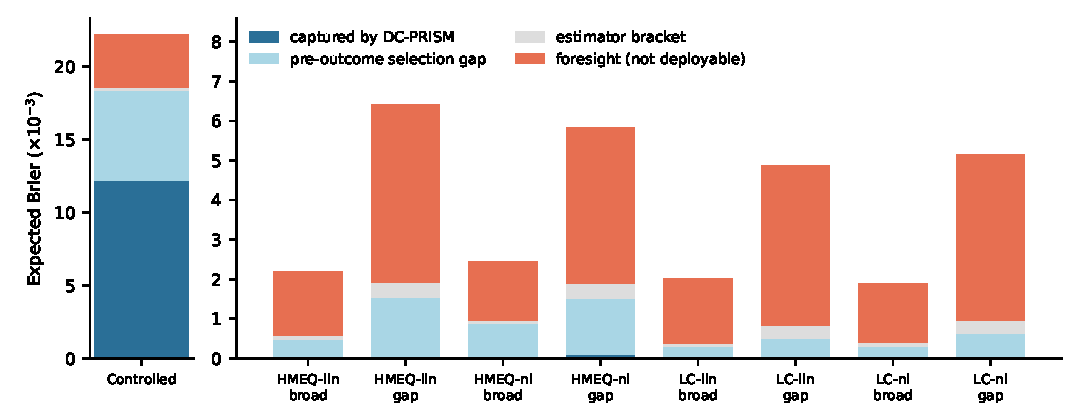
\includegraphics[width=\linewidth]{figures/supplement_v3_opportunity.pdf}
 \caption{结果后提升空间的分解~\eqref{eq:opportunity}。灰色：$H_{\mathrm{pre}}$ 的插值估计与交叉拟合估计之间的差距。左：受控世界；右：真实协变量各臂（lin/nl 为结果模型，broad/gap 为历史类型）。注意纵轴尺度不同。}
 \label{fig:opportunity}
\end{figure}

\paragraph{定位结果前差距。}DC-PRISM 在每个臂中的事前收益都在 $\pm0.1\times10^{-3}$ 以内，因此其选择差距几乎等于全部 $H_{\mathrm{pre}}$。为了定位这一差距，我们分别在拟合参数 $\widehat\theta$ 和总体参数 $\theta_{\mathrm{pop}}$（真实 $p$ 在逻辑模型类上的 KL 投影，在逻辑设置中等于真实参数）处，用 $V_\theta$ 对同一集合族排序。在真实协变量上，参数效应（$\theta_{\mathrm{pop}}$ 处收益减去 $\widehat\theta$ 处收益，均值 $0.02$--$0.61$）与剩余近似差距（$H_{\mathrm{pre}}$ 减去 $\theta_{\mathrm{pop}}$ 处收益，均值 $0.09$--$0.40$）在 16 个注册检验中均不显著（$\times10^{-3}$）。在覆盖缺口下，代理对集合族的排序良好（$\rho=0.55$--$0.69$），选择其最大值者可在全部四种缺口设置中获取交叉拟合 $H_{\mathrm{pre}}$ 的 41--54\%（表~\ref{tab:realx}）。在受控世界中情形相反：代理的排序没有信息量（$\rho\approx0$），在 $\theta_{\mathrm{pop}}$ 处排序比在 $\widehat\theta$ 处显著\emph{更差}（$-11.2$，区间 $[-15.7,-6.6]$），且近似差距是实质性的（$18.9$，$[14.2,23.5]$），这与逻辑模型类错误设定的辅助尾部机制相一致。

\paragraph{保守性权衡。}综合以上结果，我们提出如下机制；由于它结合了注册终点与描述性比较，我们将其标注为探索性结论。在局部代理不可靠之处（如错误设定的受控尾部），DC-PRISM 的相对基准、低分位数、带阻尼的比较将无信息量的排序转化为较大收益（$12.2$，而代理最大值者为 $4.9$）。在代理可靠之处（如带覆盖缺口的真实协变量），同样的保守性使其在 84--95\% 的状态中保留基准集合，从而放弃了代理单独即可获取的那部分 $H_{\mathrm{pre}}$。与此一致的是，门限与数量惩罚在真实协变量上几乎不起作用，而该处单个常数的最大影响来自阻尼与分位数，但均低于 $0.25\times10^{-3}$。真实协变量上涉及的绝对数值很小：在我们的设置中最多只有 $1.9\times10^{-3}$ Brier 是可部署的。

\section{真实标签上的延迟回放}
\label{sec:replay}
\paragraph{协议。}我们在经过处理的 HMEQ、LendingClub、PPDai 和 UCI Credit 队列上回放十轮，使用六个特征和记录的二元结果~\cite{sasHMEQ,lendingclubSource,ppdaiSource,yeh2009comparison}。每个种子保留 1{,}000 行测试数据、600 行目标数据和一个 600 行的历史窗口，从中抽取 68 条初始记录。每轮提供 24 个候选和 14 个常规获取。探索标签在选择后一轮到达，常规标签在两轮后到达；Brier 损失在每轮开始、到期标签释放之后测量。ALC-Brier 为十轮分数的平均。预处理在初始历史上拟合，数值预算由初始模型确定并在各策略间固定。我们使用两种候选流。\emph{工程化}流按可观测协变量排序，从狭窄的初始历史出发提供低风险、与待反馈方向一致、互补和尾部候选，与受控设计相呼应。\emph{自然}流则随机抽取初始历史以及每轮的记录。每种流在每个队列上使用 32 个新划分种子和九个策略；DC-PRISM 与七个对照策略中的每一个进行比较，构成一个包含 56 个检验的比较族。

\begin{table}[t]
\caption{延迟回放：每个队列 32 个种子上的平均 ALC-Brier（$\times10^{-2}$）。种子层面的标准差在此单位下为 0.7--3.1，比大多数策略间差异高一个数量级。}
\label{tab:replay}
\centering\small
\setlength{\tabcolsep}{3.5pt}
\begin{tabular}{lrrrrrrrr}
\toprule
& \multicolumn{4}{c}{工程化流} & \multicolumn{4}{c}{自然流} \\
\cmidrule(lr){2-5}\cmidrule(lr){6-9}
策略 & HMEQ & LC & PPDai & UCI & HMEQ & LC & PPDai & UCI \\
\midrule
仅常规获取 & 16.87 & 17.05 & 12.83 & 17.85 & 13.84 & 15.72 & 11.72 & 15.98 \\
Safe-MinRisk & 16.95 & 16.81 & 12.64 & 17.76 & 13.73 & 15.59 & 11.61 & 15.85 \\
固定数量 & 16.96 & 16.85 & 12.49 & 17.76 & 13.70 & 15.61 & 11.58 & 15.85 \\
Random & 16.81 & 16.85 & 12.58 & 17.80 & 13.73 & 15.67 & 11.62 & 15.87 \\
Uncertainty & 16.79 & 16.97 & 12.39 & 17.77 & 13.73 & 15.63 & 11.53 & 15.79 \\
Fisher-cost & 16.65 & 16.55 & 12.48 & 17.80 & 13.62 & 15.60 & 11.61 & 15.86 \\
BAIT-greedy & 16.67 & 16.54 & 12.50 & 17.83 & 13.56 & 15.62 & 11.52 & 15.82 \\
TargetVar-greedy & 16.65 & 16.57 & 12.51 & 17.82 & 13.60 & 15.60 & 11.53 & 15.82 \\
DC-PRISM & 16.66 & 16.65 & 12.35 & 17.75 & 13.67 & 15.56 & 11.55 & 15.85 \\
\bottomrule
\end{tabular}
\end{table}

\begin{figure}[t]
 \centering
 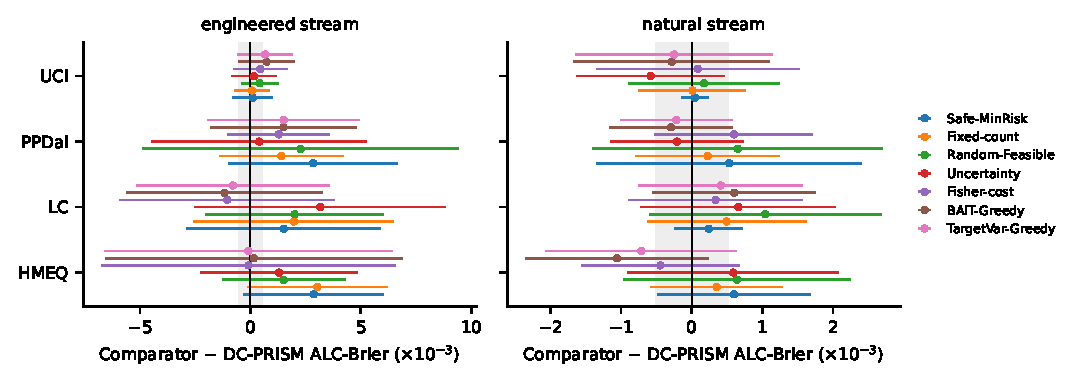
\includegraphics[width=\linewidth]{figures/supplement_v3_online.pdf}
 \caption{在 56 个检验的比较族上，对照策略减去 DC-PRISM 的 ALC-Brier 及 95\% 同时区间；正值有利于 DC-PRISM。灰色带：$\pm5\times10^{-4}$。}
 \label{fig:replay}
\end{figure}

\paragraph{结果。}56 个检验的比较族中没有任何一项比较是决定性的（图~\ref{fig:replay}）。在工程化流上，DC-PRISM 在 HMEQ、LendingClub 和 PPDai 上的均值比以数量为导向的策略（Safe-MinRisk、固定数量、Random）低 $1.4$--$3.0\times10^{-3}$，与基于信息的策略（Fisher-cost、BAIT-greedy、TargetVar-greedy）相差在 $\pm1.5\times10^{-3}$ 以内。在自然流上，所有策略与 DC-PRISM 的差距都在 $1.1\times10^{-3}$ 以内；在 UCI Credit 上，它与 Safe-MinRisk 的差异落在实质性带内。早先一批 16 个种子的实验曾发现一项实质性收益，即在 PPDai 上相对固定数量的 $4.1\times10^{-3}$；本次更大规模的研究未能复现该结果（$1.4$，区间 $[-1.4,4.2]\times10^{-3}$）。DC-PRISM 每轮获取 $3.9$--$6.5$ 个标签，BAIT-greedy 与 TargetVar-greedy 为 $2.4$--$4.6$ 个。所有受包络约束的策略在每一轮都保持在预算之内。回放结果与第~\ref{sec:realx}~节一致：在真实结果上，扣除先见之后剩余的机会很小，而利用这些机会的策略在当前样本量下在统计上无法区分。

\section{相关工作}
\label{sec:related}
\paragraph{面向预测的获取与批量获取。}主动学习选择观测以改进预测模型~\cite{cohn1996active,settles2009active}，方法涵盖不确定性采样~\cite{lewis1994sequential}，以及基于直推式设计~\cite{yu2006transductive}、Fisher 嵌入（BAIT）~\cite{ash2021fishing}、梯度多样性~\cite{ash2020badge}、联合互信息~\cite{kirsch2019batchbald}、预测信息（EPIG）~\cite{bickfordsmith2023prediction}和决策损失~\cite{huang2026loss}的准则。代价敏感与预算受限的变体处理异质的标注成本~\cite{tomanek2010cost,morato2025conbatch}。这些方法提供了我们所使用的信息几何。我们研究的对象不同：基于敞口的可行域与待反馈信息如何改变数量与组成的相对价值，以及由此产生的机会中有多少是可部署的。

\paragraph{选择性标签、安全性与延迟。}选择性标签研究形式化了仅在有利决策下才揭示结果的问题~\cite{lakkaraju2017selective}；Wei~\cite{wei2021selective}、Kilbertus 等~\cite{kilbertus2020fair}与 Keswani 等~\cite{keswani2024partial}研究了在探索与效用、公平性或覆盖之间权衡的策略，日志数据也可用于引导进一步的实验~\cite{yan2018logged}。在信用评分中，拒绝推断试图校正被拒申请者结果缺失的问题~\cite{crook2004reject}。安全探索~\cite{sui2015safe}与保守型老虎机~\cite{wu2016conservative}以安全性或基线性能要求约束探索；带延迟反馈的在线学习~\cite{joulani2013delayed,chapelle2014delayed}与考虑延迟的主动学习~\cite{pham2022latency}处理迟到的结果。我们的设定结合了这些要素，但提出了它们未单独刻画的机制性问题：在状态与风险预算固定时，哪种可行组成更有价值，以及表面优势中有多少能够在结果到达前被知晓。

\section{讨论与结论}
\label{sec:conclusion}
与实现后最优集合进行事后比较，是说明某个选择规则“把价值留在了桌上”的自然方式。我们的分解表明这种比较可能产生误导。在围绕方向性待反馈信息与错误设定尾部构建的受控世界中，大部分事后提升空间是可部署的，一种保守的、考虑待反馈信息的比较能以更少的标签获取其中大部分。在真实信贷协变量上，同样的提升空间大部分属于先见。剩余部分随覆盖缺口增大，并能被局部信息代理良好排序，但保守的决策规则未能加以利用。在线回放中，包括 DC-PRISM 在内的基于信息的策略彼此之间无法区分。

\paragraph{局限性。}真实协变量上的结果由已知概率生成，因为测量 $H_{\mathrm{pre}}$ 需要这些概率。回放使用固定的、经过处理的队列，采用随机划分而非按时间划分，我们不声称具有外部或时间上的有效性。风险包络的概率保证要求 $q$ 同时覆盖真实概率，而我们的经验分数并不能确保这一点。BAIT-greedy（仅前向步）与 TargetVar-greedy（EPIG 的 Laplace 近似）是改编版本，而非完整复现。保守性权衡是对注册终点的探索性综合。

\paragraph{展望。}结果指向两个具体方向：一是从可见信息诊断代理的可靠性，以便在代理排序良好时放松保守性；二是在评估获取规则时报告结果前提升空间，而非事后提升空间。代码、冻结协议、汇总结果与验证脚本已在匿名仓库中提供。

\bibliographystyle{splncs04}
\bibliography{refs}
\end{document}
